%%%%%%%%%%%%%%%%%%%%%%%%%%%%%%%%%%%%%%%%%
% Beamer Presentation
% LaTeX Template
% Version 1.0 (10/11/12)
%
% This template has been downloaded from:
% http://www.LaTeXTemplates.com
%
% License:
% CC BY-NC-SA 3.0 (http://creativecommons.org/licenses/by-nc-sa/3.0/)
%
%%%%%%%%%%%%%%%%%%%%%%%%%%%%%%%%%%%%%%%%%

%----------------------------------------------------------------------------------------
%    PACKAGES AND THEMES
%----------------------------------------------------------------------------------------

\documentclass{beamer}

\mode<presentation> {

% The Beamer class comes with a number of default slide themes
% which change the colors and layouts of slides. Below this is a list
% of all the themes, uncomment each in turn to see what they look like.

%\usetheme{default}
%\usetheme{AnnArbor}
%\usetheme{Antibes}
%\usetheme{Bergen}
%\usetheme{Berkeley}
%\usetheme{Berlin}
%\usetheme{Boadilla}
%\usetheme{CambridgeUS}
%\usetheme{Copenhagen}
%\usetheme{Darmstadt}
%\usetheme{Dresden}
%\usetheme{Frankfurt}
%\usetheme{Goettingen}
%\usetheme{Hannover}
%\usetheme{Ilmenau}
%\usetheme{JuanLesPins}
%\usetheme{Luebeck}
\usetheme{Madrid}
%\usetheme{Malmoe}
%\usetheme{Marburg}
%\usetheme{Montpellier}
%\usetheme{PaloAlto}
%\usetheme{Pittsburgh}
%\usetheme{Rochester}
%\usetheme{Singapore}
%\usetheme{Szeged}
%\usetheme{Warsaw}

% As well as themes, the Beamer class has a number of color themes
% for any slide theme. Uncomment each of these in turn to see how it
% changes the colors of your current slide theme.

%\usecolortheme{albatross}
%\usecolortheme{beaver}
%\usecolortheme{beetle}
%\usecolortheme{crane}
%\usecolortheme{dolphin}
%\usecolortheme{dove}
%\usecolortheme{fly}
%\usecolortheme{lily}
%\usecolortheme{orchid}
%\usecolortheme{rose}
%\usecolortheme{seagull}
%\usecolortheme{seahorse}
%\usecolortheme{whale}
%\usecolortheme{wolverine}

%\setbeamertemplate{footline} % To remove the footer line in all slides uncomment this line
%\setbeamertemplate{footline}[page number] % To replace the footer line in all slides with a simple slide count uncomment this line

%\setbeamertemplate{navigation symbols}{} % To remove the navigation symbols from the bottom of all slides uncomment this line
}

\usepackage{graphicx} % Allows including images
\usepackage{booktabs} % Allows the use of \toprule, \midrule and \bottomrule in tables

%----------------------------------------------------------------------------------------
%    TITLE PAGE
%----------------------------------------------------------------------------------------

\title[Placement Dashboard]{PLACEMENT DASHBOARD } % The short title appears at the bottom of every slide, the full title is only on the title page  

\author[Bhumika, Vaishnavi]{Bhumika Saxena, Vaishnavi Janardhan} % Your name
% \institute % Your institution as it will appear on the bottom of every slide, may be shorthand to save space
{
  % Your institution for the title page
\medskip
% \textit{bhumika056btcse17@igdtuw.ac.in} % Your email address
}
\date{\today} % Date, can be changed to a custom date

\begin{document}

\begin{frame}
\titlepage % Print the title page as the first slide
\end{frame}

\begin{frame}
\frametitle{ ~ Our objective} 
\begin{itemize}
\item{Enhancing knowledge of Python}
\item{Exploring Python frameworks}
\item{Delving into web technologies} 
\end{itemize}
\end{frame}

\begin{frame}
\frametitle{~ Description}
\begin {itemize}
\item{Placement data of TalentSprint}
\item{Pictorial representation of data}
\item{Easy analysis}
\end{itemize}
\end{frame}

\begin{frame}
\frametitle{ ~ Technology Stack} 
\begin {itemize}
\item Front-end
    \begin {itemize}
        \item{HTML} 
        \item{CSS}
        \item{JavaScript}
    \end{itemize}
\bigskip 
\item Back-end
    \begin {itemize}
        \item{Python} 
        \item{Python frameworks}
    \end{itemize}
\bigskip 
\item Database Management
    \begin {itemize}
        \item{MySQL}
    \end{itemize}
\end{itemize}
\end{frame}

\begin{frame}
\frametitle{ ~ Aim for the project week} 
\begin{itemize}
\item{Building dashboard using Django}
\item{Enhancing UI/UX}
\end{itemize}
\end{frame}

\begin{frame}
\frametitle{ ~ Current progress}
\begin{center}
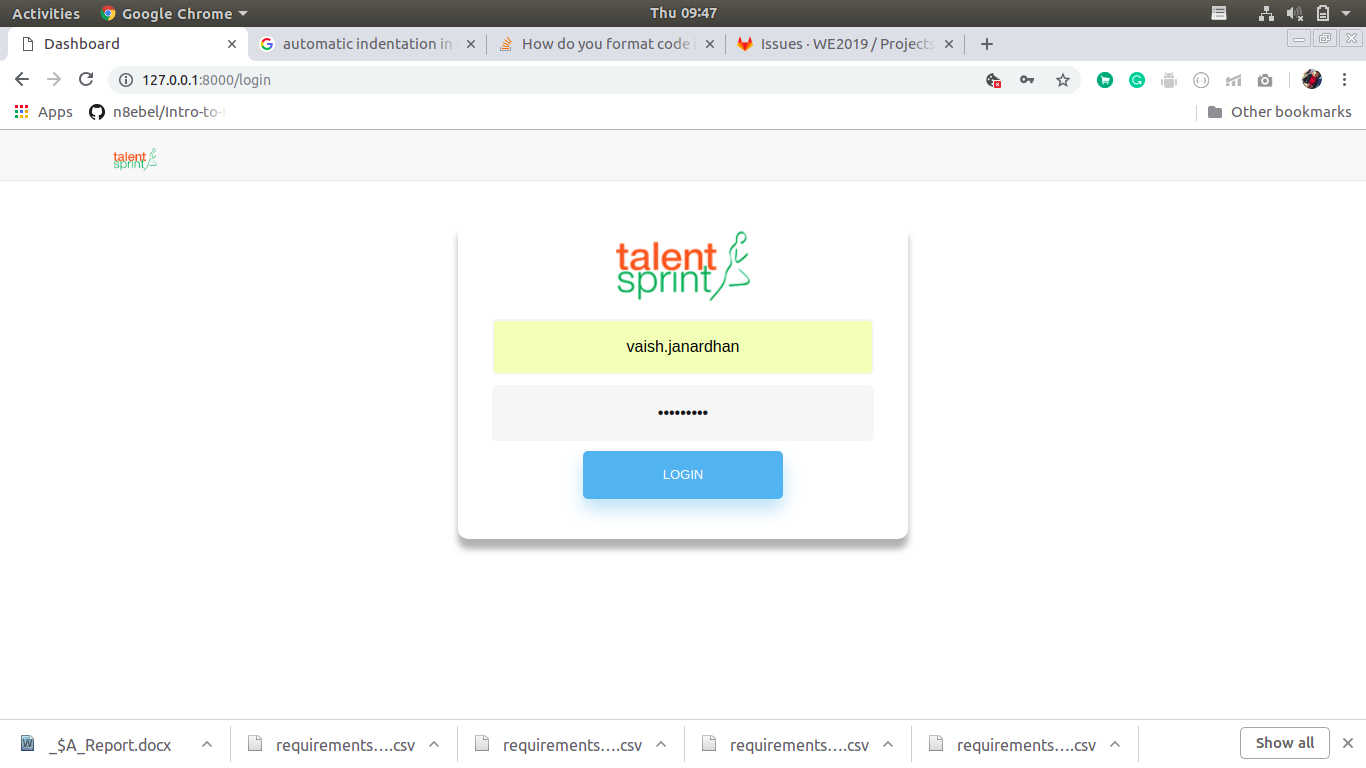
\includegraphics[width = 10cm]{1.png}
\end{center}
\end{frame}

\begin{frame}
\frametitle{ ~ Current progress}
\begin{center}
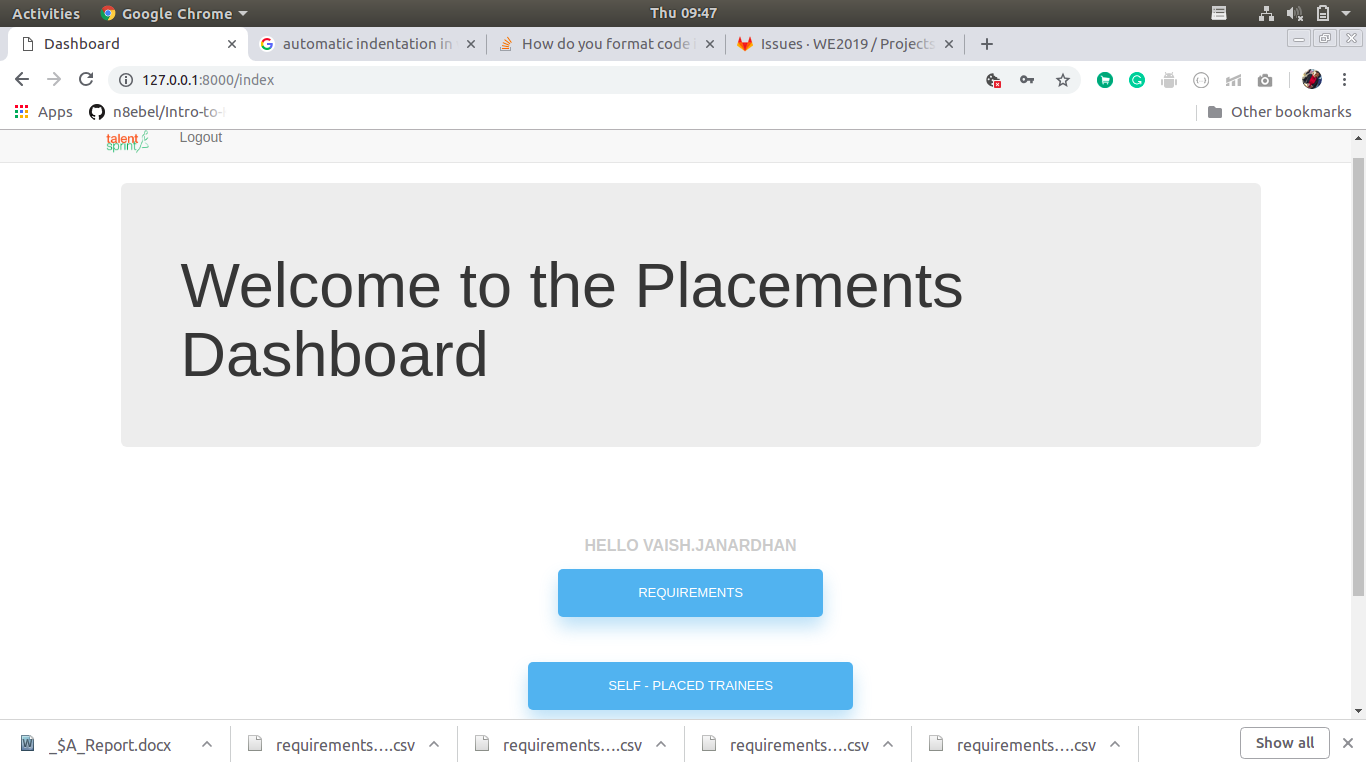
\includegraphics[width = 10cm]{2.png}
\end{center}
\end{frame}

\begin{frame}
\frametitle{ ~ Aim for today}
\begin{center}
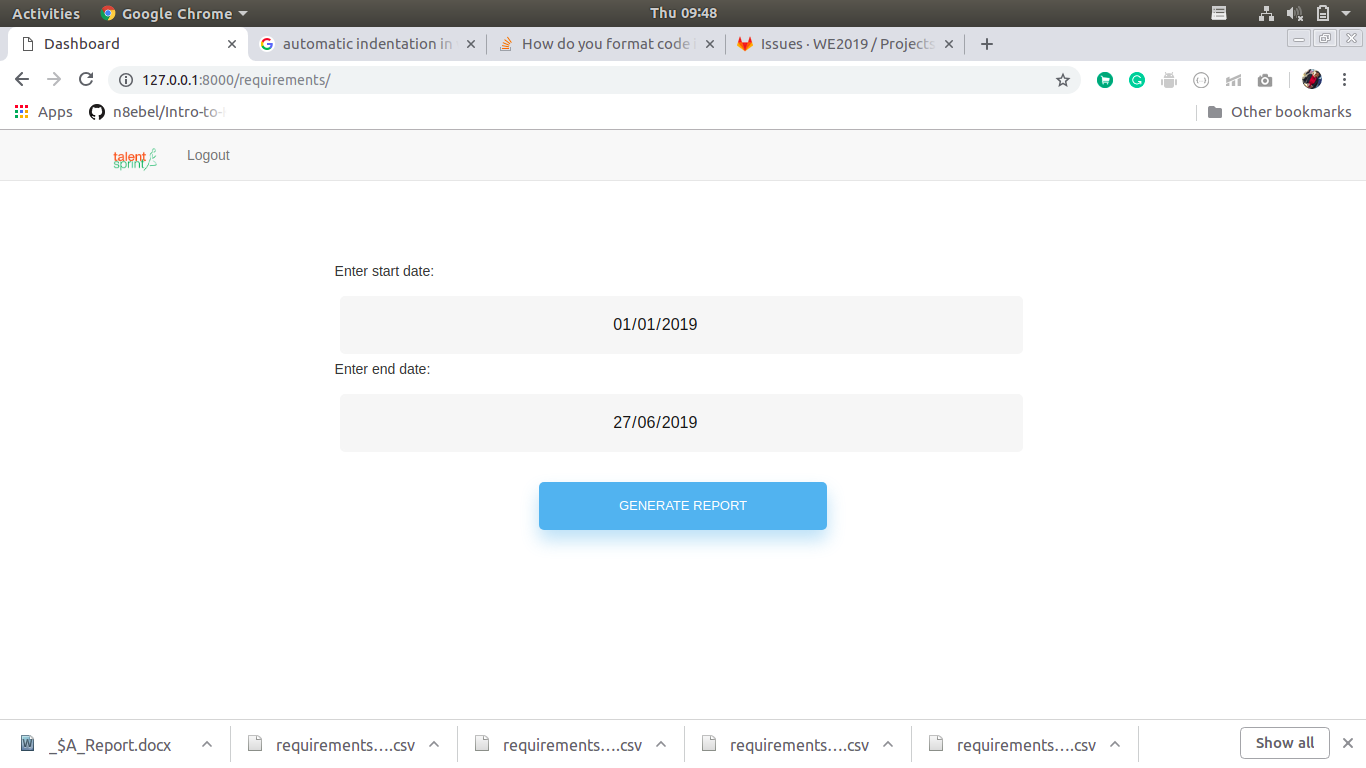
\includegraphics[width = 10cm]{3.png}
\end{center}
\end{frame}



\begin{frame}
\frametitle{~ Timeline}
\begin{center}

\begin{tabular}{|l|l|}
     \hline
     June 23 & Initial Setup\\
     \hline
     June 24 & Preparing the front-end skeleton\\
     \hline & Studying the database\\
     \hline
     June 25 & Connecting to database\\
     \hline & Showing response in tables\\
     \hline
     June 26 & Visualization using D3.js and Canvas\\
     \hline
     June 27 onwards & Extension to other modules\\
     \hline
     
\end{tabular}
\end{center}    
\end{frame}

\begin{frame}
\frametitle{ ~ Future Prospect} 
\begin{itemize}
\item{Using Pyramid}
\item{Comparing frameworks}
\item{Generating a detailed report}
\end{itemize}
\end{frame}


%------------------------------------------------

\begin{frame}
\begin{center}
\Huge{Discussion}
\end{center}
\end{frame}

%----------------------------------------------------------------------------------------

\end{document}